\documentclass{article}

\usepackage{amsmath}
\usepackage{amssymb}
\usepackage{amsthm}
\usepackage{authblk}
\usepackage[english]{babel}
\usepackage{blkarray}
\usepackage[font=small]{caption}
\usepackage{cite}
\usepackage{graphicx}

% ---- Author affiliations ---- %

\renewcommand\Affilfont{\itshape\small}

% ---- Propositions, lemmas, defintions... ---- %

\newtheorem{algorithm}{Algorithm}
\newtheorem{corollary}{Corollary}
\newtheorem{definition}{Definition}
%\newtheorem{example}{Example}
\newtheorem{lemma}{Lemma}
\newtheorem{proposition}{Proposition}
%\newtheorem{remark}{Remark}


% ---- Special environments (examples and remarks) ---- %

\newcounter{examplecounter}
\newenvironment{example}
{\small\vspace{0.5\baselineskip}
  \refstepcounter{examplecounter}%
  \noindent\textbf{Example \arabic{examplecounter}.}%
}{\vspace{-0.2\baselineskip}\begin{center}%
  $\star$\end{center}\vspace{0.5\baselineskip}}

\newcounter{remarkcounter}
\newenvironment{remark}
{\small\it\vspace{0.5\baselineskip}
  \refstepcounter{remarkcounter}%
  \noindent\textbf{Remark \arabic{remarkcounter}.}%
}{\vspace{0.5\baselineskip}}

\newenvironment{inset}
{\vspace{0.5\baselineskip}\begin{center}}
{\end{center}\vspace{0.5\baselineskip}}


% ---- Macros ---- %

\newcommand{\DN}{\scriptstyle{\Downarrow}}
\newcommand{\dn}{\scriptstyle{\downarrow}}
\newcommand{\up}[1]{\scriptstyle{(\uparrow)_{#1}}}
\newcommand{\eq}[1]{\scriptstyle{(\sim)_{#1}}}

\newcommand{\upg}{\scriptstyle{\uparrow}}
\newcommand{\eqg}{\scriptstyle{\sim}}

%---------------------------------------------------------------

\title{Calibrating MEM seeding heuristics}

\author[1,2]{Guillaume J. Filion}
\affil[1]{Genome Architecture, Gene Regulation, Stem Cells and Cancer
Programme, Center for Genomic Regulation (CRG), The Barcelona Institute of
Science and Technology, Dr. Aiguader 88, Barcelona 08003, Spain.}
\affil[2]{University Pompeu Fabra, Doctor Aiguader, 08003 Barcelona,
Spain.}

\date{\today}

%---------------------------------------------------------------
%---------------------------------------------------------------


\begin{document}

\maketitle

\begin{abstract}
The abstract will come later.
\end{abstract}


%---------------------------------------------------------------
%---------------------------------------------------------------

\section{Introduction}
Some introduction

\section{MEM seeds}

\subsection{Seeds}
DEFINE MEM SEED AND SHARED MEM SEED.

\subsection{The seeding alphabet}

By nature, reads are sequences of \texttt{A}, \texttt{T}, \texttt{G} and
\texttt{C}, but for the purpose of the seeding process, it is more useful
to consider them as a sequence of symbols telling if the nucleotides match
the target and~/ or the duplicates. Here, we will consider that reads are
sequences of the five symbols $\Downarrow$, $\downarrow$, $\uparrow$, $\sim$
and $\square$.

The $\Downarrow$ symbol indicates that the nucleotide is not only a
mismatch for the target, but also for every duplicate. The $\downarrow$
symbol indicates that the nucleotide is a mismatch for the target, but is
a match for at least one dupulicate. These two symbols are referred to as
the \emph{error symbols}, because they imply the occurrence of a
sequencing error (this is the only way the read may not match the target).

The remaing three symbols have a more complex usage because they describe
events of the MEM seeding process that are best explained by way of a
concrete example. Fig.~\ref{fig:sketch_MEM} illustrates the case of a read
of size 25 from a sequence with three duplicates. The four files of
squares at the bottom are the target and duplicate sequences, where a
black square means that the decoded nucleotide is a mismatch and a grey
square means that it is a match.


\begin{figure}[h]
\centering
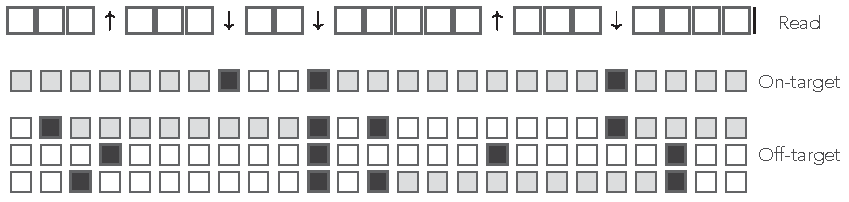
\includegraphics[scale=.9]{sketch_MEM.pdf}
\caption{\textbf{Reads and MEM seeds}. 
Some legend.}
\label{fig:sketch_MEM}
\end{figure}

Now consider streaks of matches until a particular position of the read.
At the 4-th nucleotide, the target scores 4 matches in a row versus 2, 0
and 1 for the duplicates. The target just acquired the strictly longest
streak, which is indicated by the $\uparrow$ symbol. This symbol also
appears at position 17, where the target sequence acquires the strictly
longest streak again (6 matches in a row, versus 4, 0 and 4 for the
dupicates).

At position 23, the target and the first duplicate both acquire the
longest streak (2 matches in a row), which is indicated by the $\sim$
symbol. This symbol is used only at positions where the target
\emph{acquires} the longest streak (together with at least one duplicate).
For instance, it is not used at position 1 nor at position 12 because the
target already had the longest streak (0 in both cases).

Finally, the $\square$ symbol is used for all the other cases,
\textit{i.e.}, when there is no sequencing error, and when the target does
not acquire the longest streak of matches (shared or not with a
duplicate).

Each sequence corresponds to a Bernoulli process where `success' stands
for a match between the sequence and the read, and `failure' stands for a
mismatch. For simplicity, we will refer to the Bernoulli processes as
`threads'.

\begin{definition}
At a given position of the read, a duplicate thread is said to be
\emph{strictly masking} if its match streak is strictly longer than the
match streak of the target. A duplicate thread is said to be
\emph{potentially masking} if its match streak is the same as the target.
\end{definition}

Duplicate threads are thus classified into strictly masking, potentially
masking and not masking, which allows us to describe the usage of the five
symbols.

\begin{figure}[h]
\centering
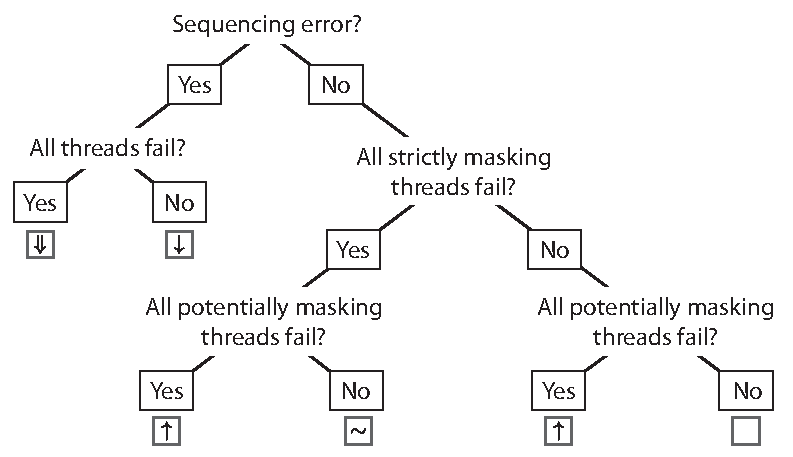
\includegraphics[scale=.7]{decision_tree.pdf}
\caption{\textbf{Decision tree}. 
Some legend.}
\label{fig:decision_tree}
\end{figure}


We assume that the target sequence has $N$ duplicates that are potential
false positives for the seeding process. We further assume that
duplication was instantaenous and that all $N+1$ sequences diverge
independently from each other at a constant rate. In other words, we
ignore the complications due to the genealogy of the duplication events
and we simply assume that at each position, any given duplicate has the
same nucleotide as the target with probability $1-\mu$. If it does not,
we assume that the duplicate has any of the remaining three
nucleotides with equal probability.

To describe those processes, we will
often use the function $\varphi(n)$ that gives the length of the success
streak at position $n$. The processes are indexed such that $\varphi_0$
refers to the target sequence, and functions $\varphi_j$ $(1 \leq j \leq
N)$ refer to the duplicates. For a concrete example, $\varphi_0(5) = 5$
and $\varphi_1(5) = 3$ in Fig.~\ref{fig:sketch_MEM}.



With these definitions, the decision tree for choosing the next symbol to
insert in a read can be summarized as in Fig.~\ref{fig:decision_tree}.
This sketch will be useful as a reference to compute the probabilities of
the blocks and their weighted generating functions.




\begin{definition}
The main thread is dominant at nucleotide $n$ if $\varphi_0(n) >
\varphi_i(n)$ for all $i$ $(1 \leq i \leq N)$. The main thread is
co-dominant if inequality is not strict and there exists $i$ $(1\leq i
\leq N)$ such that $\varphi_0(n) = \varphi_i(n)$.
\end{definition}



\begin{figure}[h]
\centering
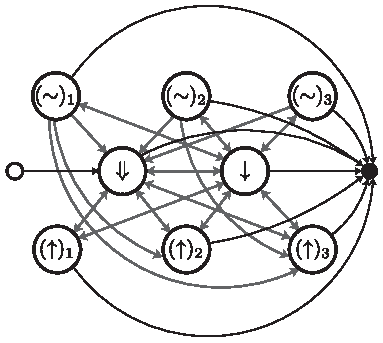
\includegraphics[scale=1]{no_3MEM_graph.pdf}
\caption{\textbf{Transfer graph of a read without 3-MEM}. 
Some legend.}
\label{fig:noMEM_graph}
\end{figure}



\section{The transfer matrix}

\subsection{Transitions from $\uparrow$}
\label{sec:trans_from_up}

On a $\uparrow$ symbol, the main thread becomes dominant. It will remain
so until the first sequencing error, so the next block will be terminated
by an error symbol (\textit{i.e.} $\Downarrow$ or $\downarrow$).

\begin{definition}
$\omega$ and $\tilde{\omega}$ are the probabilities of the $\Downarrow$
and of the $\downarrow$ error symbols, respectively, \textit{i.e.}
\begin{eqnarray}
\omega &=& p \cdot (1-\mu/3)^N \\
\tilde{\omega} &=& p \cdot \big( 1-(1-\mu/3)^N \big).
\end{eqnarray}
\end{definition}

The weighted generating function of the transition from $(\uparrow)_j$ to
$\Downarrow$ is
\begin{equation}
D_{\gamma-j}(z) = \omega z \sum_{i=0}^{\gamma-j-1} (qz)^i.
\end{equation}

The weighted generating function of the transition from
$(\uparrow)_j$ to $\downarrow$ is
\begin{equation}
\tilde{D}_{\gamma-j}(z) = \tilde{\omega} z
  \sum_{i=0}^{\gamma-j-1} (qz)^i.
\end{equation}


\subsection{Transitions from $\Downarrow$}
\label{sec:trans_from_Down}

At a $\Downarrow$ symbol, all the threads have match length $0$ and the
read is `reset' to its initial state. The main thread is co-dominant with
all the alternative threads. The next terminator symbol depends on what
happens first. If all the alternative threads fail before the main thread,
the latter becomes dominant ($\uparrow$ symbol). If not all alternative
threads have failed when the main thread does, we need to distinguish two
cases: if all threads fail together with the main thread, the read is
reset ($\Downarrow$ symbol), otherwise the main read becomes dominated
($\downarrow$ symbol).

If the next terminator is the $\uparrow$ symbol, we need to distinguish
the cases based on the value of $\varphi_0$ (see
section~\ref{sec:trans_from_up}), which is just the position of the
$\uparrow$ symbol after the $\Downarrow$ symbol in this case. A transition
from $\Downarrow$ to $(\uparrow)_j$ consists of a succession of $j$
correct nucleotides -- each with probability $q$. But we must also make
sure that no other $\uparrow$ symbol is inserted before position $j$.

\begin{definition}
$\xi_{i,m}$ is the probability that at least one of $m$ alternative
threads does not fail in $i$ nucleotides, \textit{i.e.}
\begin{equation}
  \xi_{i,m} = 1-(1-(1-\mu)^i)^m.
\end{equation}
\end{definition}

The weighted generating function of the transition from $\Downarrow$ to
$(\uparrow)_i$ is
\begin{equation}
u_i(z) = (\xi_{i-1,N}-\xi_{i,N})(qz)^i.
\end{equation}


If the next terminator is $\Downarrow$, there is a limit on the
number of $\square$ symbols. Indeed, if there are $\gamma$ or more
nucleotides between the two $\Downarrow$ symbols, they constitute a shared
MEM seed. As mentioned in section~\ref{sec:trans_from_up}, the weighted
generating function of the $\Downarrow$ symbol is $pz(1-\mu/3)^N$. By the
same rationale as above, the weighted generating function of the
transition from $\Downarrow$ to $\Downarrow$ is
\begin{equation}
A_{\gamma}(z) = \omega z
  \sum_{i=0}^{\gamma-1} \xi_{i,N} \cdot (qz)^i.
\end{equation}


If the next terminator is $\downarrow$, there is no limit on the number of
$\square$ symbols that can be inserted. Indeed, the main thread will not
be part of the MEM in this case. As mentioned in
section~\ref{sec:trans_from_up}, the weighted generating function of the
$\downarrow$ symbol is $pz(1-(1-\mu/3)^N)$. The probability that it first
occurs at position $n+1$ after the $\Downarrow$ symbol is the probability
that the first $n$ nucleotides are correct -- each with probability $q$
-- and that at least one alternative thread survives -- probability
$\xi_{n,N}$. The weighted generating function of the transition from
$\Downarrow$ to $\downarrow$ is thus
\begin{equation}
\tilde{A}_\infty(z) = \tilde{\omega} z
  \sum_{i=0}^\infty \xi_{i,N} \cdot (qz)^i.
\end{equation}

\subsection{Transitions from $\downarrow$}
\label{sec:trans_from_down}

At a $\downarrow$ symbol, the main thread fails and at least one duplicate
thread does not (othwerwise the symbol would be $\Downarrow$). By
definition, the duplicate threads that do not fail are strictly masking,
and those that fail are potentially masking. A $\downarrow$ symbol implies
the presence of a sequencing error, so duplicate threads fail with
probability $1-\mu/3$. The probability that $m$ duplicate threads fail and
$N-m$ do not $(0 \leq m \leq N-1)$ is thus
\begin{equation}
  Q_m = \frac{1}{1-(1-\mu/3)^N}{N \choose m} (1-\mu/3)^m(\mu/3)^{N-m}.
\end{equation}

The $\downarrow$ symbol can be followed by all the terminators. We need to
start with the case of the $\sim$ terminator, because it will be required
for the other ones. Referring to the decision tree of
Fig.~\ref{fig:decision_tree}, we see that the $\sim$ symbol occurs in an
error-free stretch, if all the strictly masking threads fail before the
potentially masking threads. In section~\ref{sec:trans_from_sim} it will
be important to distinguish different cases based on the value of
$\varphi_0$ at the position of the $\sim$ symbol, so as in
section~\ref{sec:trans_from_up}, we introduce the states $(\sim)_j$ $(1
\leq j \leq \gamma-1)$ such that $\varphi_0(n) = j$ if the nucleotide at
position $n$ is $(\sim)_j$. In this case, the value of $\varphi_0(n) = j$
is simply the position of the $\sim$ symbol relative to the preceding
$\downarrow$ symbol.

If there are $m = 0$ potentially masking threads, the next terminator
cannot be $\sim$. Assuming that there are $m > 0$ potentially masking
threads at the $\downarrow$ symbol, the probability that the have not all
faied at position $i$ is $\xi_{i,m}$. Similarly, the probability that the
last strictly masking thread fails at position $i$ is
$\xi_{i-1,N-m}-\xi_{i,N-m}$. So the probability that the next terminator
is $(\sim)_i$ is $q^j V_i$, where
\begin{eqnarray}
\label{eq:Si}
V_i &=& \sum_{m=0}^{N-1} Q_m \cdot \xi_{i,m} \cdot
  (\xi_{i-1,N-m}-\xi_{i,N-m}) \notag \\
  &=& \frac{\alpha_i^N-\alpha_{i-1}^N-\gamma_i^N+\delta_{i-1}^N}
{1-(1-\mu/3)^N} \text{, where}
\end{eqnarray}

\begin{eqnarray}
\alpha_i &=& 1-(1-\mu)^i\mu/3 \\
\gamma_i &=& 1-(1-\mu)^i \\
\delta_i &=& 1-(1-\mu+\mu^2/3)(1-\mu)^i.
\end{eqnarray}

We have assumed $m>0$, but the sum above can start at $m=0$ because
$\xi_{i,0}=0$. So the weighted generating function of the transition from
$\downarrow$ to $(\sim)_i$ is
\begin{equation}
v_i(z) = \frac{\alpha_i^N-\alpha_{i-1}^N-
  \gamma_i^N+\delta_{i-1}^N}{1-(1-\mu/3)^N} \cdot (qz)^i.
\end{equation}

Referring again to the decision of Fig.~\ref{fig:decision_tree}, we see
that the $\uparrow$ symbol occurs in an error-free stretch, if all the
potentially masking threads fail before or at the same nucleotide as the
strictly masking threads. Assuming that there are $m \geq 0$ potentially
masking threads at the $\downarrow$ symbol, the probability that they have
all failed at position $i$ is $1-\xi_{i,m}$. As we have seen above, the
probability that the last strictly masking thread fails at position $j$ is
$\xi_{i-1,N-m}-\xi_{i,N-m}$. So the probability that the next terminator
is the $\uparrow$ symbol at position $i$ is $q^i W_i$, where
\begin{eqnarray}
  W_i &=& \sum_{m=0}^{N-1} Q_m \cdot (1-\xi_{i,m}) \cdot
  (\xi_{i-1,N-m}-\xi_{i,N-m}) \notag \\
    &=& \frac{\gamma_i^N-\delta_{i-1}^N}{1-(1-\mu/3)^N}.
\end{eqnarray}

The weighted generating function of the transition from $\downarrow$ to
$(\uparrow)_i$ is
\begin{equation}
w_i(z) = \frac{\gamma_i^N- \delta_{i-1}^N}{1-(1-\mu/3)^N} \cdot (qz)^i.
\end{equation}

In order to compute the weighted generating functions of the other
transitions, first observe that
\begin{equation}
V_j+W_j = \frac{\alpha_j^N - \alpha_{j-1}^N}{1-(1-\mu/3)^N}.
\end{equation}
So the probability that an error-free stretch of length $i \geq 1$
following a $\downarrow$ symbol contains neither a $\sim$ symbol nor a
$\uparrow$ symbol is
\begin{equation}
\sum_{j=1}^i V_j+W_j = \frac{\alpha_i^N -
\alpha_0^N}{1-(1-\mu/3)^N}.
\end{equation}

The probability that the next terminator after a $\downarrow$ symbol is a
$\Downarrow$ symbol at position $j$ is the probability of an error-free
stretch of size $j-1$ that contains neither the $\sim$ symbol nor the
$\uparrow$ symbol -- probability as above multiplied by $q^j$ -- followed
by a $\Downarrow$ symbol -- probability $pz(1-\mu/3)^N$. Thus, the
weighted generating function of the transition from $\downarrow$ to
$\Downarrow$ is
\begin{equation}
B_\infty(z) = \omega z \cdot \Big(1 + \sum_{i=1}^\infty
\frac{\alpha_i^N - \alpha_0^N}{1-(1-\mu/3)^N} (qz)^i \Big).
\end{equation}

By the same rationale, we see that the weighted generating function of the
transition from $\downarrow$ to $\downarrow$ is
\begin{equation}
\tilde{B}_\infty(z) = \tilde{\omega} z \cdot \Big(1 + \sum_{i=1}^\infty
\frac{\alpha_i^N - \alpha_0^N}{1-(1-\mu/3)^N} (qz)^i \Big).
\end{equation}

\subsection{Transitions from $\sim$}
\label{sec:trans_from_sim}

At a $\sim$ symbol, the main thread becomes co-dominant, together with $1$
to $N-1$ alternative threads (if there were $N$, the symbol would be
$\Downarrow$). As in section~\ref{sec:trans_from_Down}, the next
terminator symbol depends on whether all the alternative co-dominant
threads fail before the main thread. If this is the case, the main thread
will become dominant ($\uparrow$ symbol), otherwise we again need to
distinguish the case that the read is reset ($\Downarrow$ symbol) from the
case that the main thread becomes dominated ($\downarrow$ symbol).

An important difficulty is that the $\sim$ symbol does not inform us about
the number of surviving threads (except when $N = 1$). So we need to
marginalize the probabilities of interest over this number. The first
thing to note is that a $\sim$ terminator can only follow a $\downarrow$
terminator. Indeed, after a $\Downarrow$ symbol the threads are already
co-dominant, and after a $\uparrow$ symbol the alternative threads cannot
`catch up' with the main thread until a sequencing error occurs,
\textit{i.e.} until a $\Downarrow$ symbol or a $\downarrow$ symbol is
inserted. The number of surviving threads depends on the position of the
$\sim$ symbol relative to the preceding $\downarrow$ symbol, so we need
to treat the states $(\sim)_j$ separately.

We first establish an equality that will turn out to be useful in the
subsequent calculations.

\begin{lemma}
For any real numbers $x$ and $y$,
\begin{eqnarray*}
\sum_{n=m}^N {N \choose n} {n \choose m} x^n y^{N-n}
&=& x^m \sum_{r=0}^{N-m} {N \choose m+r} {m+r \choose m}a^r y^{N-m-r} \\
&=& {N \choose m} x^m \sum_{r=0}^{N-m} {N-m \choose r}x^r y^{N-m-r} \\
&=& {N \choose m} x^m (x+y)^{N-m}.
\end{eqnarray*}

The equality above implies
\begin{equation}
\label{eq:double_binom}
\sum_{n=m}^{N-1} {N \choose n} {n \choose m} x^n y^{N-n} =
{N \choose m} x^m \Big[ (x+y)^{N-m} - x^{N-m} \Big].
\end{equation}
\end{lemma}

The probability that there are $m>1$ potentially masking threads upon
entering state $(\sim)_j$ is the probability that there were $n \geq m$
potentially masking threads at the $\downarrow$ symbol -- probability
$Q_n$ --, that exactly $m$ have survived until position $j$ -- probability
${n \choose m} (1-\mu)^{jm} (1-(1-\mu)^j)^{n-m}$ -- and that the last of
the $N-n$ strictly masking threads fails at position $j$ -- probability
$\xi_{j-1,N-n}-\xi_{j,N-n}$. Summing over $n = m, \ldots, N-1$, the
probability is seen to be
\begin{equation}
\label{eq:miscprob}
\sum_{n=m}^{N-1} Q_n \cdot {n \choose m} (1-\mu)^{jm} (1-(1-\mu)^j)^{n-m}
\cdot (\xi_{j-1,N-n}-\xi_{j,N-n}).
\end{equation}

We write $\xi_{j-1,N-n}-\xi_{j,N-n}$ as $(1-\xi_{j,N-n}) -
(1-\xi_{j-1,N-n})$ and split the sum of equation (\ref{eq:miscprob}) into
two parts. The first term is equal to
\begin{equation*}
\begin{split}
\sum_{n=m}^{N-1} & Q_n \cdot {n \choose m} (1-\mu)^{jm} (1-(1-\mu)^j)^{n-m}
\cdot (1 - \xi_{j,N-n}) = \\
& \frac{(1-\mu)^{jm} (1-(1-\mu)^j)^{N-m}}{1-(1-\mu/3)^N}
\sum_{n=m}^{N-1} {N \choose n} {n \choose m} (1-\mu/3)^n (\mu/3)^{N-n}.
\end{split}
\end{equation*}

Using formula (\ref{eq:double_binom}) with $x=1-\mu/3$ and $y=\mu/3$, we
see that this term is equal to
\begin{equation*}
\frac{(1-\mu)^{jm} (1-\mu/3)^m}{1-(1-\mu/3)^N} {N \choose m} 
\bigg( \gamma_j^{N-m}
-\big[ (1-(1-\mu)^j)(1-\mu/3)\big]^{N-m} \bigg).
\end{equation*}

The second term of equation (\ref{eq:miscprob}) is equal to
\begin{multline*}
\sum_{n=m}^{N-1} Q_n \cdot {n \choose m} (1-\mu)^{jm} (1-(1-\mu)^j)^{n-m}
\cdot (1 - \xi_{j-1,N-n}) = \\
\frac{1}{1-(1-\mu/3)^N}
\left(\frac{(1-\mu)^j}{1-(1-\mu)^j}\right)^m
\; \sum_{n=m}^{N-1} {N \choose n} {n \choose m} \times \\
(1-\mu/3)^n (\mu/3)^{N-n}
(1-(1-\mu)^j)^n (1-(1-\mu)^{j-1})^{N-n}.
\end{multline*}

Formula (\ref{eq:double_binom}) with $x=(1-(1-\mu)^j)(1-\mu/3)$ and
$y = (1-(1-\mu)^{j-1})\mu/3$ yields
\begin{equation*}
\frac{(1-\mu)^{jm} (1-\mu/3)^m}{1-(1-\mu/3)^N} {N \choose m}
\bigg( \delta_{j-1}^{N-m}
-\big[ (1-(1-\mu)^j)(1-\mu/3)\big]^{N-m} \bigg).
\end{equation*}

Computing the difference between the terms, we see that the probability
that there are $m$ potentially masking threads upon entering state
$(\sim)_j$ is
\begin{equation*}
P_{m,j} = \frac{(1-\mu)^{jm} (1-\mu/3)^m}{1-(1-\mu/3)^N} {N \choose m} 
\big( \gamma_j^{N-m} - \delta_{j-1}^{N-m} \big).
\end{equation*}


The sum of the terms above for $m = 1, \ldots, N-1$ is $V_j$ from equation
(\ref{eq:Si}), which is the probability of the $(\sim)_j$ terminator.

Now, referring to the decision tree of Fig.~\ref{fig:decision_tree}, we
see that if the $m$ potentially masking threads fail before the main
thread, the next terminator will be the $\uparrow$ symbol, otherwise it
will be either the $\Downarrow$ symbol or the $\downarrow$ symbol.

The probability that the last of the $m$ potentially masking threads fails
at position $i$ after entering state $(\sim)_j$ is
$\xi_{i-1,m}-\xi_{i,m}$. Dividing by $V_j$ and summing over $m = 1,
\ldots, N-1$, we find that the weighted generating function of the
transition from $(\sim)_j$ to $(\uparrow)_{j+i}$ is
\begin{eqnarray}
y_{j,j+i}(z) &=& \sum_{m=1}^{N-1} \frac{P_{m,j}}{V_j}
\big( \xi_{i-1,m}-\xi_{i,m} \big) (qz)^i \notag \\
&=& \frac{\beta_{j,i+j}^N - \beta_{j,i+j-1}^N
-\beta_{j-1,i+j}^N + \beta_{j-1,i+j-1}^N}
  {\alpha_j^N-\alpha_{j-1}^N-\gamma_j^N+\delta_{j-1}^N} (qz)^i,
\end{eqnarray}
where $\alpha_j$, $\delta_j$, $\gamma_j$ are as above, and where
\begin{equation}
\beta_{j,i} = 1 - (1-\mu)^j\mu/3 + (1-\mu)^i(1-\mu/3).
\end{equation}

The probability that the next terminator is a $\Downarrow$ symbol or a
$\downarrow$ symbol at position $i$ is the probability that at least one
of the potentially masking threads survives until position $i-1$ --
probability $\xi_{i-1,m}$ -- and that the next nucleotide is a sequencing
error -- probability $p$. Dividing by $V_j$ and summing over $m = 1,
\ldots, N-1$, we find that the weighted generating function of the
transtion from $(\sim)_j$ to
$\Downarrow$ is
\begin{eqnarray}
C_{\gamma-j}(z) &=& \omega z \sum_{i=1}^{\gamma-j-1} \sum_{m=1}^{N-1}
  \frac{P_{m,j}}{V_j} \xi_{i-1,m} \cdot (qz)^{i-1} \notag \\
  &=& \omega z \sum_{i=1}^{\gamma-j-1}
\frac{ \alpha_j^N-\alpha_{j-1}^N-\beta_{j,i+j-1}^N
  +\beta_{j-1,i+j-1}^N }
{\alpha_j^N-\alpha_{j-1}^N-\gamma_j^N+\delta_{j-1}^N} (qz)^{i-1}.
\end{eqnarray}

With the same notations, the weighted generating function from $(\sim)_j$
to $\downarrow$ is seen to be 
\begin{equation}
\tilde{C}_{\gamma-j}(z) = \tilde{\omega} z \sum_{i=1}^{\gamma-j-1}
\frac{ \alpha_j^N-\alpha_{j-1}^N-\beta_{j,i+j-1}^N
  +\beta_{j-1,i+j-1}^N }
{\alpha_j^N-\alpha_{j-1}^N-\gamma_j^N+\delta_{j-1}^N} (qz)^{i-1}.
\end{equation}

\subsection{Head and tail vectors}

At the beginning of the read, the match lengths of all the threads are
$0$. This is exactly the same as on a $\Downarrow$ symbol. We can thus
consider that the read starts in the $\Downarrow$ state, which is
equivalent to adding an edge labelled with the empty object $\varepsilon$
between the head vertex and the $\Downarrow$ vertex. The head vector is
thus
\begin{equation*}
H(z) = 
\begin{blockarray}{cccccccc}
   \;\; \DN & \dn &\eq{1} & \ldots & \eq{\gamma-1} &
    \up{1} & \ldots & \up{\gamma-1} \\
\begin{block}{[cccccccc]}
\;\; 1 & 0 & 0 & \ldots & 0 & 0 & \ldots & 0 \\
\end{block}
\end{blockarray}.
\end{equation*}
The tail vector contains the weighted generating functions of
non-terminated stretches of $\square$ symbols. Referring to the decision
tree of Fig.~\ref{fig:decision_tree}, we see that the probability of
occurrence of $\square$ symbols depends on whether there are potentially
masking and / or strictly masking threads. All the symbols except
$\downarrow$ impose a maximum on the number of $\square$ symbols at the
end of the reads.

For the $\downarrow$ symbol, the weighted generating function is simply
\begin{equation}
T_{\downarrow}(z) = \sum_{i=0}^\infty (qz)^i = \frac{1}{1-qz}.
\end{equation}

For the $(\uparrow)_j$ state, the weighted generating function is
\begin{equation}
T_{(\uparrow)_j}(z) = \sum_{i=0}^{\gamma-j-1} (qz)^i.
\end{equation}

For the other symbols, we must take care that the potentially masking
threads do not all fail (otherwise this would imply the presence of a
$\uparrow$ terminator in the tail). For the $\Downarrow$ symbol, the
weighted generating function is
\begin{equation}
T_{\Downarrow}(z) = \sum_{i=0}^{\gamma-1} \xi_{i,N} \cdot (qz)^i.
\end{equation}

For the $(\sim)_j$ state, the weighted generating function is
\begin{equation}
T_{(\sim)_j}(z) = \sum_{i=0}^{\gamma-j-1}
\frac{ \alpha_j^N-\alpha_{j-1}^N-\beta_{j,i+j}^N +\beta_{j-1,i+j}^N }
{\alpha_j^N-\alpha_{j-1}^N-\gamma_j^N+\delta_{j-1}^N} (qz)^i.
\end{equation}

In summary,
\begin{equation*}
T(z) = 
\begin{blockarray}{cc}
\begin{block}{c[c]}
\dn & T_\downarrow(z) \\
\DN & T_\Downarrow(z) \\
\eq{1} & T_{(\sim)_1}(z) \\
\vdots & \vdots \\
\eq{\gamma-1} & T_{(\sim)_{\gamma-1}}(z) \\
\up{1} & T_{(\uparrow)_1}(z) \\
\vdots & \vdots \\
\up{\gamma-1} & \; T_{(\uparrow)_{\gamma-1}}(z) \; \\
\end{block}
\end{blockarray}.
\end{equation*}


\section{Conclusion}

\begin{equation*}
\begin{blockarray}{ccccccccc}
   & \DN & \dn &\eq{1} & \ldots & \eq{\gamma-1} &
    \up{1} & \ldots & \up{\gamma-1} \\
\begin{block}{c[cccccccc]}
\DN & A_\gamma(z) & \tilde{A}_\infty(z) & 0 & \ldots & 0 & u_1(z)
    & \ldots & u_{\gamma-1}(z) \\
\dn & B_\infty(z) & \tilde{B}_\infty(z) & v_1(z) & \ldots &
    v_{\gamma-1}(z) & w_1(z) & \ldots & w_{\gamma-1}(z) \\
\eq{1} & C_{\gamma-1}(z) & \tilde{C}_{\gamma-1}(z) & 0 & \ldots & 0 & 0 &
    \ldots & y_{1,\gamma-1}(z) \\
\eq{2} & C_{\gamma-2}(z) & \tilde{C}_{\gamma-2}(z) & 0 & \ldots & 0 & 0 &
    \ldots & y_{2,\gamma-1}(z) \\
\vdots & \vdots & \vdots & \vdots & \ddots & \vdots & \vdots &
    \ddots & \vdots \\
\eq{\gamma-1} & C_1(z) & \tilde{C}_1(z) & 0 & 
    \ldots & 0 & 0 & \ldots & 0 \\
\up{1} & D_{\gamma-1}(z) & \tilde{D}_{\gamma-1}(z) & 0 & \ldots & 0 & 0 &
    \ldots & 0 \\
\up{2} & D_{\gamma-2}(z) & \tilde{D}_{\gamma-2}(z) & 0 & \ldots & 0 & 0 &
    \ldots & 0  \\
\vdots & \vdots & \vdots & \vdots & \ddots & \vdots & \vdots &
    \ddots & \vdots \\
\up{\gamma-1} & D_1(z) & \tilde{D}_1(z) & 0 & \ldots & 0 & 0 &
    \ldots & 0 \\
\end{block}
\end{blockarray}
\end{equation*}


\section*{Acknowledgements}

I acknowledge the financial support of the Spanish Ministry of Economy and
Competitiveness (‘Centro de Excelencia Severo Ochoa 2013-2017’, Plan
Nacional BFU2012-37168), of the CERCA Programme~/~Generalitat de
Catalunya, and of the European Research Council (Synergy Grant 609989).


%---------------------------------------------------------------
%---------------------------------------------------------------

\bibliography{references,pubmed}
\bibliographystyle{plain}

%----------------------------------------------------------------

\end{document}

%gs -dNoOutputFonts -sDEVICE=pdfwrite -o out.pdf latex.pdf 
